
\usetikzlibrary{arrows.meta}
\tikzset{
    myptr/.style={-{Stealth[scale=3]}},
}
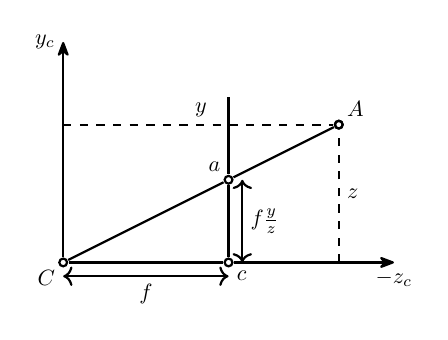
\begin{tikzpicture}[scale=1, every node/.style={scale=0.8}, every path/.style={scale=0.7, thick}]

    % Coordinate system
    \draw[shorten >=2pt, shorten <=2pt] (0,0) -- (3,0);
    \draw[-{Stealth[round]}, shorten <=2pt] (3,0) -- (6,0) node[anchor=north] {$-z_c$};
    \draw[-{Stealth[round]}, shorten <=2pt] (0,0) -- (0,4) node[anchor=east] {$y_c$};


    % Camera
    \node[anchor=north east] at (0,0) {$C$};
    \draw (0,0) circle (2pt);
    % line from C to A
    \draw[shorten >=2pt, shorten <=2pt] (0,0) -- (3,1.5);
    \draw (5,2.5) circle (2pt);
    \node[anchor=south east] at (3,1.5) {$a$};
    \draw (3,1.5) circle (2pt);
    \draw[shorten >=2pt, shorten <=2pt] (3,1.5) -- (5,2.5);
    \node[anchor=south west] at (5,2.5) {$A$};
    \draw (5,2.5) circle (2pt);

    % x line
    \draw[dashed, shorten >=2pt] (5,0) -- node[right] {$z$} (5,2.5);
    % y line
    \draw[dashed, shorten >=2pt] (0,2.5) -- node[above] {$y$} (5,2.5);

    % f line
    \draw[<->] (3,-0.25) -- node[below] {$f$} (0,-0.25);
    % z line
    % \draw[<->] (0,-0.2) -- node[below, xshift=12mm] {$z$} (5,-0.2);


    % Image plane
    \draw[shorten <=2pt, shorten >=2pt] (3,0) -- (3,1.5);
    \draw[shorten <=2pt] (3,1.5) -- (3,3);

%    principal point
    \draw (3,0) circle (2pt);
    \node[anchor=north west] at (3,0)  {$c$};

    % fY/Z line
    \draw[<->] (3.25,0) -- node[right] {$f\frac{y}{z}$} (3.25,1.5);
%    \draw[dashed] (2.75, 1.5) -- (3.5, 1.5);


\end{tikzpicture}